\documentclass[../main/main.tex]{subfiles}

\begin{document}

\newpage

\chapter{Design}
\section{System Architecture}
In this section, I will lay out the overall logic, and an overview of the steps involved in running my program. By decomposing the program into individual abstracted stages, I can focus on the workings and functionality of each section individually, which makes documenting and coding each section easier. I have also included a flowchart to illustrate the logic of each screen of the program.

I will also create an abstracted GUI prototype in order to showcase the general functionality of the user experience, while acting as a reference for further stages of graphical development. It will consist of individually drawn screens for each stage of the program, as shown in the top-level overview. The elements and layout of each screen are also documented below.

The following is a top-level overview of the logic of the program:

\begin{figure}[H]
    \centering
    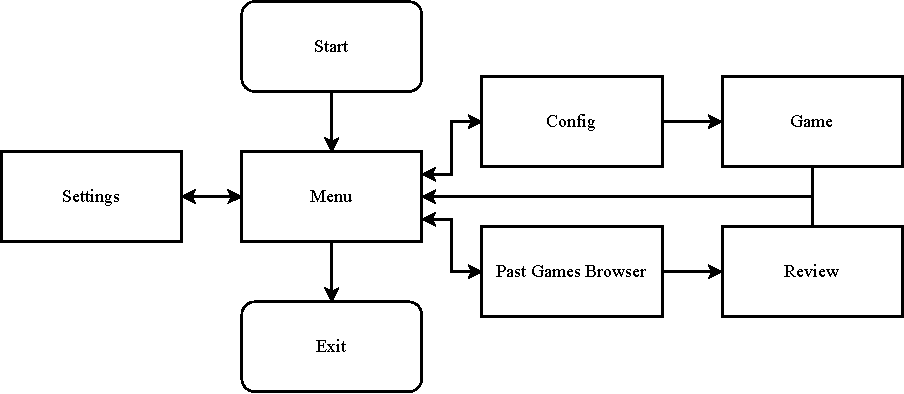
\includegraphics[width=\columnwidth]{../design/assets/top_level_overview_flowchart.pdf}
    \caption{Flowchart for Program Overview}
    \label{fig:program-overview-flowchart}
\end{figure}

\subsection{Main Menu}
\begin{figure}[H]
    \centering
    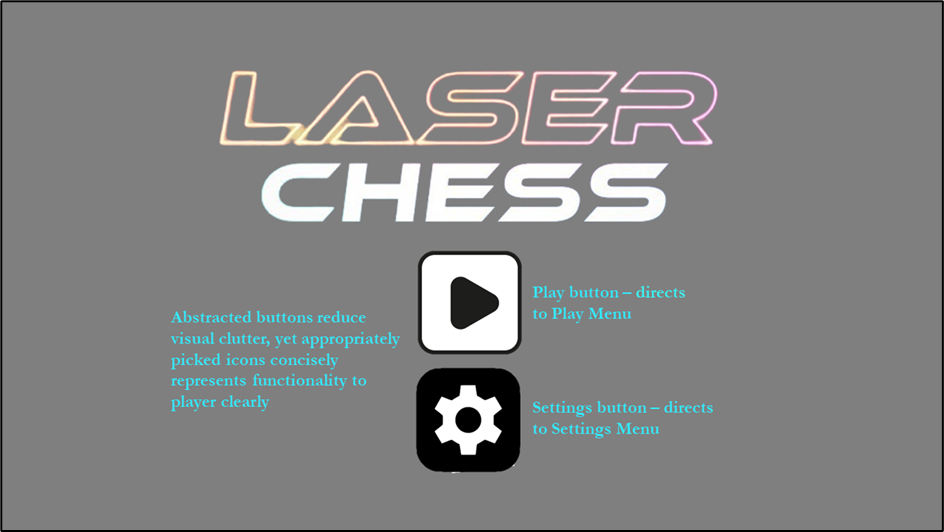
\includegraphics[width=0.8\columnwidth]{../design/assets/menu_gui.png}
    \caption{Main Menu screen prototype}
    \label{fig:menu-gui}
\end{figure}

The main menu will be the first screen to be displayed, providing access to different stages of the game. The GUI should be simple yet effective, containing clearly-labelled buttons for the user to navigate to different parts of the game.

\subsection{Settings}
\begin{figure}[H]
    \centering
    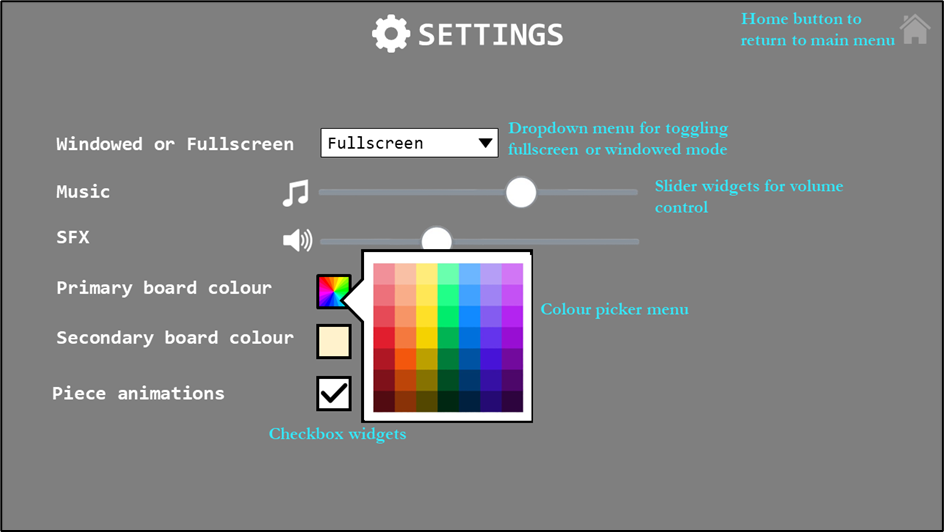
\includegraphics[width=0.8\columnwidth]{../design/assets/settings_gui.png}
    \caption{Settings screen prototype}
    \label{fig:settings-gui}
\end{figure}

The settings menu allows for the user to customise settings related to the program as a whole. The settings will be changed via GUI elements such as buttons and sliders, offering the ability to customise display mode, volume, board colour etc. Changes to settings will be stored in an intermediate code class, then stored externally into a JSON file. Game settings will instead be changed in the Config screen.

The setting screen should provide a user-friendly interface for changing the program settings intuitively; I have therefore selected appropriate GUI widgets for each setting:

\begin{itemize}
\item Windowed or Fullscreen - Drop-down list for selecting between pre-defined options
\item Music and SFX - Slider for selecting audio volume, a continuous value
\item Board colour - Colour grid for the provision of multiple pre-selected colours
\item Piece animation - Checkbox for toggling between on or off
\end{itemize}

Additionally, each screen is provided with a home button icon on the top right (except the main menu), as a shortcut to return to the main menu.

\begin{figure}[H]
    \centering
    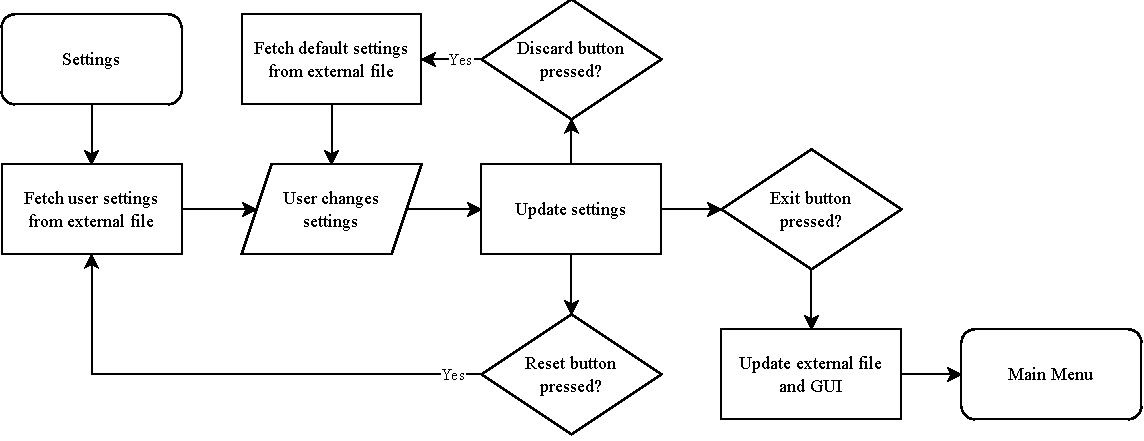
\includegraphics[width=\columnwidth]{../design/assets/settings_flowchart.pdf}
    \caption{Flowchart for Settings}
    \label{fig:settings-flowchart}
\end{figure}

\subsection{Past Games Browser}
\begin{figure}[H]
    \centering
    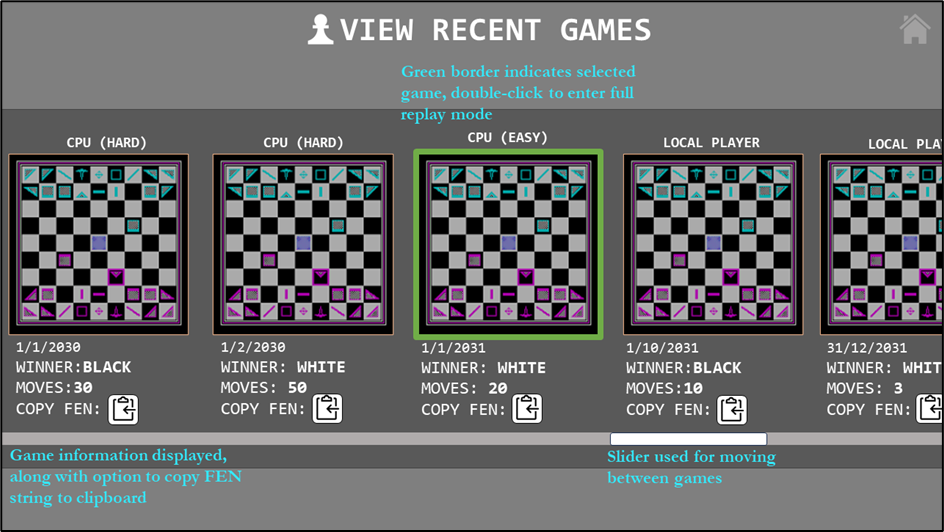
\includegraphics[width=0.8\columnwidth]{../design/assets/browser_gui.png}
    \caption{Browser screen prototype}
    \label{fig:browser-gui}
\end{figure}

The Past Games Browser menu displays a list of previously played games to be replayed. When selecting a game, the replay will render out the saved FEN string into a board position identical to the one played previously, except the user is limited to replaying back and forth between recorded moves. The menu also offers the functionality of sorting games in terms of time, game length etc.

For the GUI, previous games will be displayed on a strip, scrolled through by a horizontal slider. Information about the game will be displayed for each instance, along with the option to copy the FEN string to be stored locally or to be entered into the Review screen. When choosing a past game, a green border will appear to show the current selection, and double-clicking enters the user into the full replay mode.
While replaying the game, the GUI will appear identical to an actual game. However, the user will be limited to scrolling throughout the moves via the left and right arrow keys.

\begin{figure}[H]
    \centering
    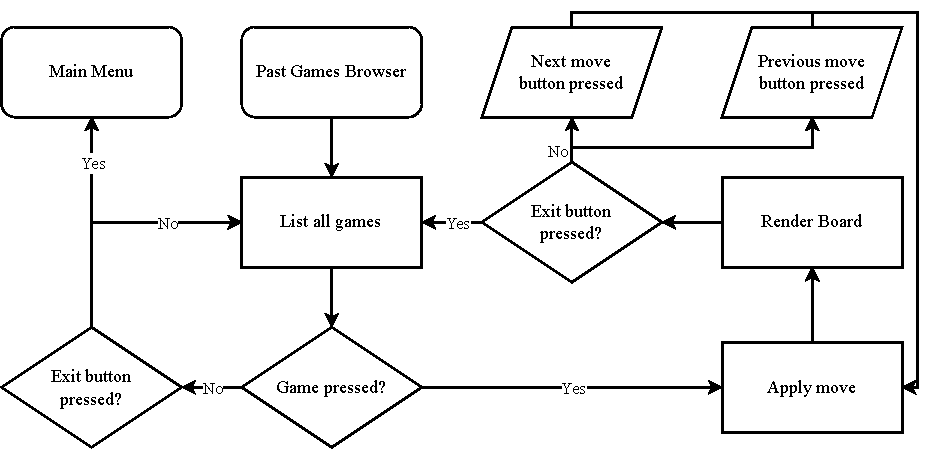
\includegraphics[width=\columnwidth]{../design/assets/browser_flowchart.pdf}
    \caption{Flowchart for Browser}
    \label{fig:browser-flowchart}
\end{figure}

\subsection{Config}
\begin{figure}[H]
    \centering
    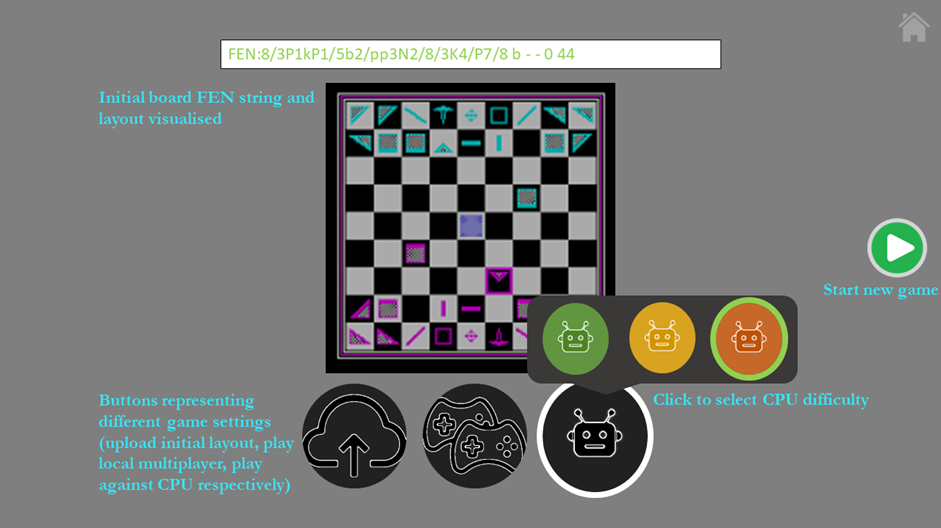
\includegraphics[width=0.8\columnwidth]{../design/assets/config_gui.png}
    \caption{Config screen prototype}
    \label{fig:config-gui}
\end{figure}

The config screen comes prior to the actual gameplay screen. Here, the player will be able to change game settings such as toggling the CPU player, time duration, playing as white or black etc.

The config menu is loaded with the default starting position. However, players may enter their own FEN string as an initial position, with the central board updating responsively to give a visual representation of the layout. Players are presented with the additional options to play against a friend, or against a CPU, which displays a drop-down list when pressed to select the CPU difficulty.

\begin{figure}[H]
    \centering
    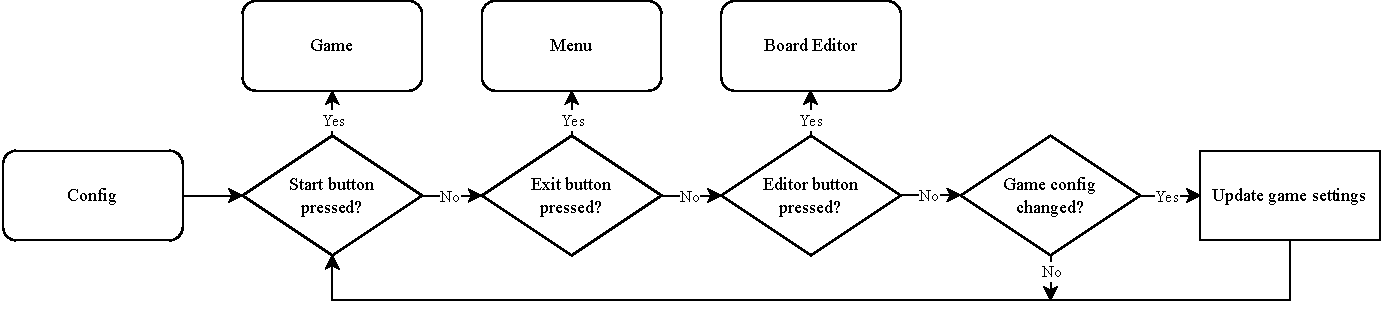
\includegraphics[width=\columnwidth]{../design/assets/config_flowchart.pdf}
    \caption{Flowchart for Config}
    \label{fig:config-flowchart}
\end{figure}

\subsection{Game}
\begin{figure}[H]
    \centering
    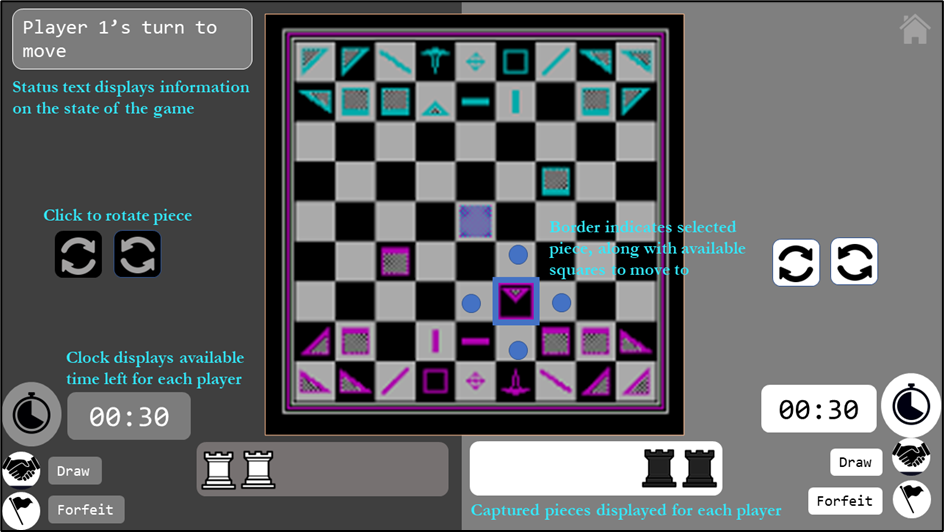
\includegraphics[width=0.8\columnwidth]{../design/assets/game_gui.png}
    \caption{Game screen prototype}
    \label{fig:game-gui}
\end{figure}

During the game, handling of the game logic, such as calculating player turn, calculating CPU moves or laser trajectory, will be computed by the program internally, rendering the updated GUI accordingly in a responsive manner to provide a seamless user experience.

In the game screen, the board is positioned centrally on the screen, surrounding by accompanying widgets displaying information on the current state of the game. The main elements include:

\begin{itemize}
\item Status text - displays information on the game state and prompts for each player move
\item Rotation buttons - allows each player to rotate the selected piece by 90° for their move
\item Timer - displays available time left for each player
\item Draw and forfeit buttons - for the named functionalities, confirmed by pressing twice
\item Piece display - displays material captured from the opponent for each player
\end{itemize}

Additionally, the current selected piece will be highlighted, and the available squares to move to will also contain a circular visual cue. Pieces will either be moved by clicking the target square, or via a drag-and-drop mechanism, accompanied by responsive audio cues. These implementations aim to improve user-friendliness and intuitiveness of the program.

\begin{figure}[H]
    \centering
    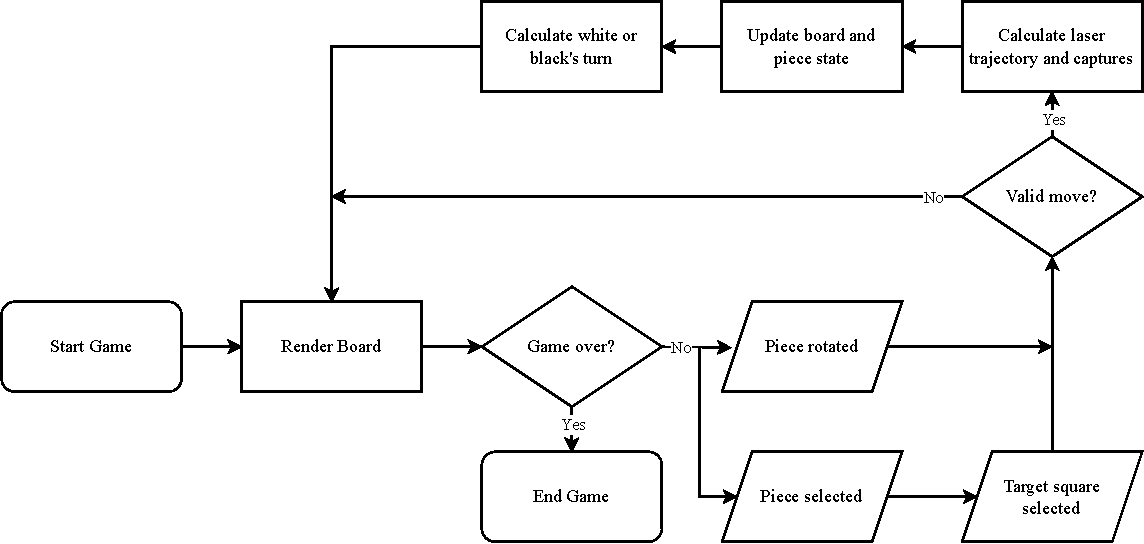
\includegraphics[width=\columnwidth]{../design/assets/game_flowchart.pdf}
    \caption{Flowchart for Game}
    \label{fig:game-flowchart}
\end{figure}

\subsection{Board Editor}
\begin{figure}[H]
    \centering
    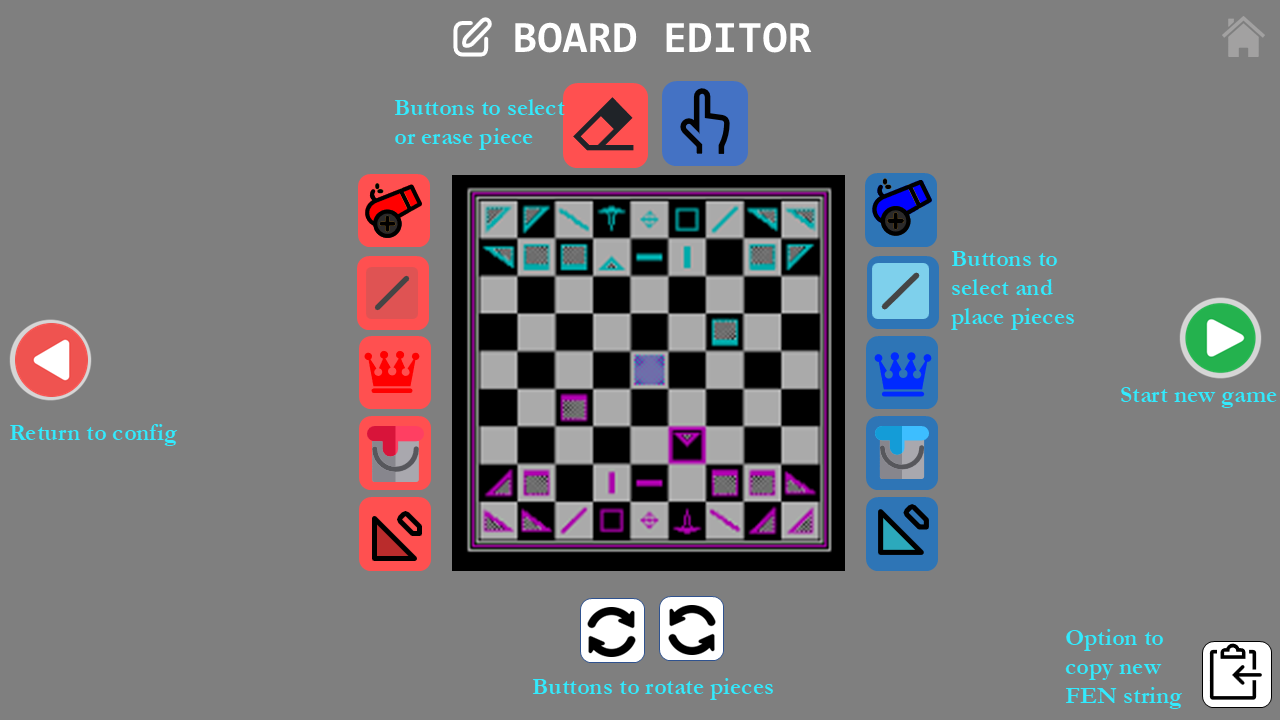
\includegraphics[width=0.8\columnwidth]{../design/assets/editor_gui.png}
    \caption{Editor screen prototype}
    \label{fig:editor-gui}
\end{figure}

The editor screen is used to configure the starting position of the board. Controls should include the ability to place all piece types of either colour, to erase pieces, and easy board manipulation shortcuts such as dragging pieces or emptying the board.

For the GUI, the buttons should clearly represent their functionality, through the use of icons and appropriate colouring (e.g. red for delete).

\begin{figure}[H]
    \centering
    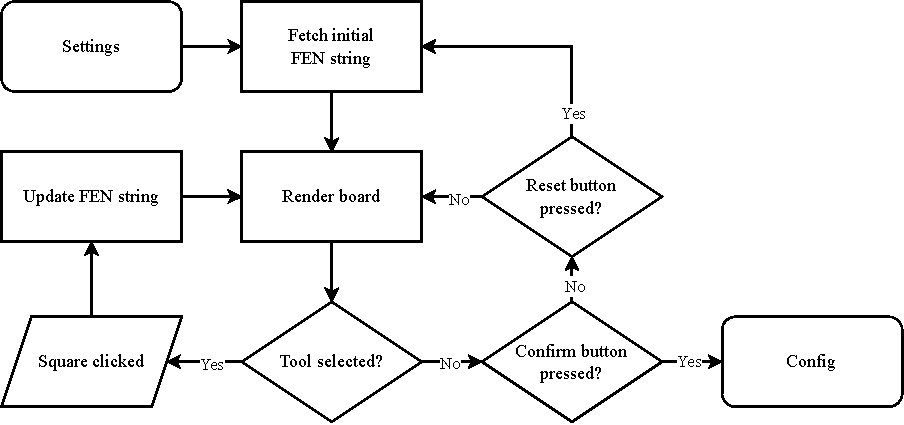
\includegraphics[width=\columnwidth]{../design/assets/editor_flowchart.pdf}
    \caption{Flowchart for board editor}
    \label{fig:editor-flowchart}
\end{figure}

\section{Algorithms and Techniques}
\subsection{Minimax}
\label{sec:design-minimax}
Minimax is a backtracking algorithm commonly used in zero-sum games used to determine the score according to an evaluation function, after a certain number of perfect moves. Minimax aims to minimize the maximum advantage possible for the opponent, thereby minimizing a player’s possible loss in a worst-case scenario. It is implemented using a recursive depth-first search, alternating between minimizing and maximising the player’s advantage in each recursive call.

\begin{figure}[H]
    \centering
    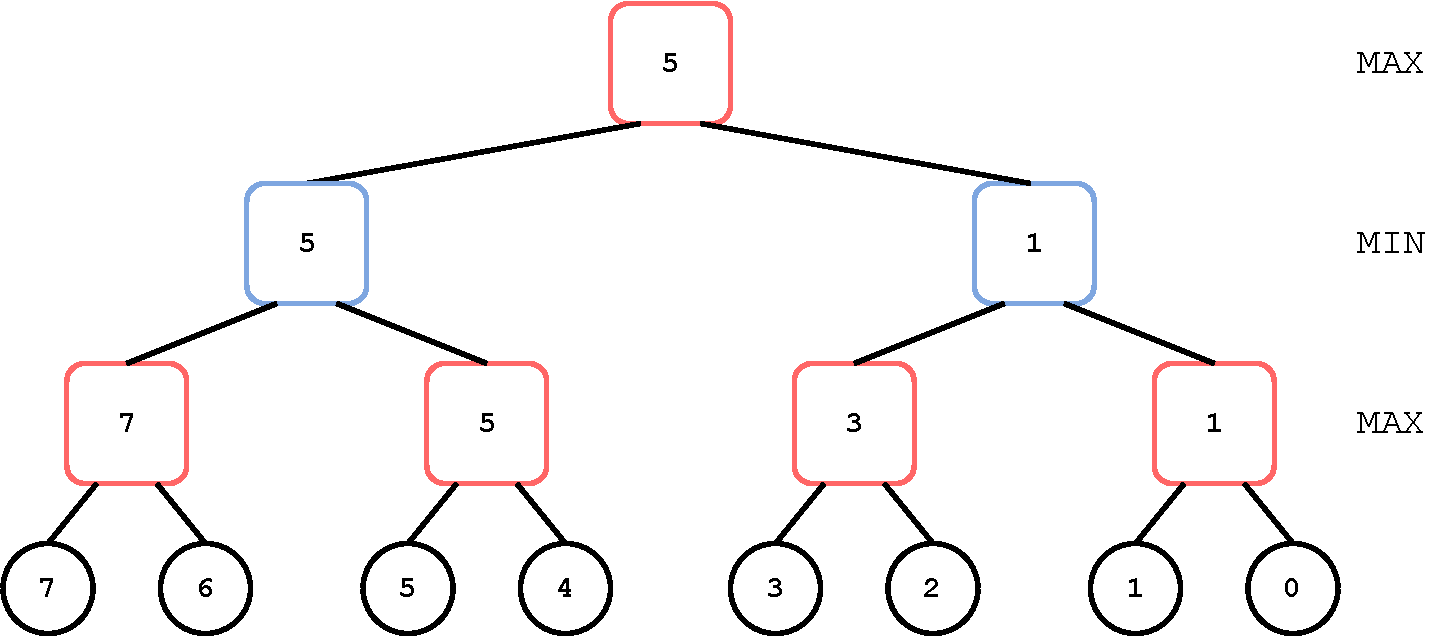
\includegraphics[width=\columnwidth]{../design/assets/minimax.pdf}
    \caption{Example minimax tree}
    \label{fig:minimax}
\end{figure}

For the example minimax tree show in Figure \ref{fig:minimax}, starting from the bottom leaf node evaluations, the maximising player would choose the highest values (7, 5, 3, 1). From those values, the minimizing player would choose the lowest values (5, 1). The final value chosen by the maximum player would therefore be the highest of the two, 5.
\\
Implementation in the form of pseudocode is shown below:

\begin{algorithm}[H]
\caption{Minimax pseudocode}
\begin{algorithmic}
    \Function{minimax}{node, depth, maximisingPlayer}
        \If{$depth = 0$ \textbf{OR} node equals game over}
            \State \Return{\Call{evaluate}{}}
        \EndIf

        \bigskip

        \If{maximisingPlayer}
            \State $value \gets -\infty$
            \For{child of node}
                \State $value \gets \Call{max}{value, \Call{minimax}{child, depth - 1, false}}$
            \EndFor
            \State \Return{$value$}
        \Else
            \State $value \gets +\infty$
            \For{child of node}
                \State $value \gets \Call{min}{value, \Call{minimax}{child, depth - 1, true}}$
            \EndFor
            \State \Return{$value$}
        \EndIf
    \EndFunction
\end{algorithmic}
\end{algorithm}

\subsection{Minimax improvements}
\subsubsection*{Alpha-beta pruning}
\label{sec:design-ab}
Alpha-beta pruning is a search algorithm that aims to decrease the number of nodes evaluated by the minimax algorithm. Alpha-beta pruning stops evaluating a move in the game tree when one refutation is found in its child nodes, proving the node to be worse than previously-examined alternatives. It does this without any potential of pruning away a better move.
The algorithm maintains two values: alpha and beta. Alpha ($\alpha$), the upper bound, is the highest value that the maximising player is guaranteed of; Beta ($\beta$), the lower bound, is the lowest value that the minimizing player is guaranteed of. If the condition $\alpha\geq\beta$ for a node being evaluated, the evaluation process halts and its remaining children nodes are ‘pruned’.
\\
This is shown in the following maximising example:

\begin{figure}[H]
    \centering
    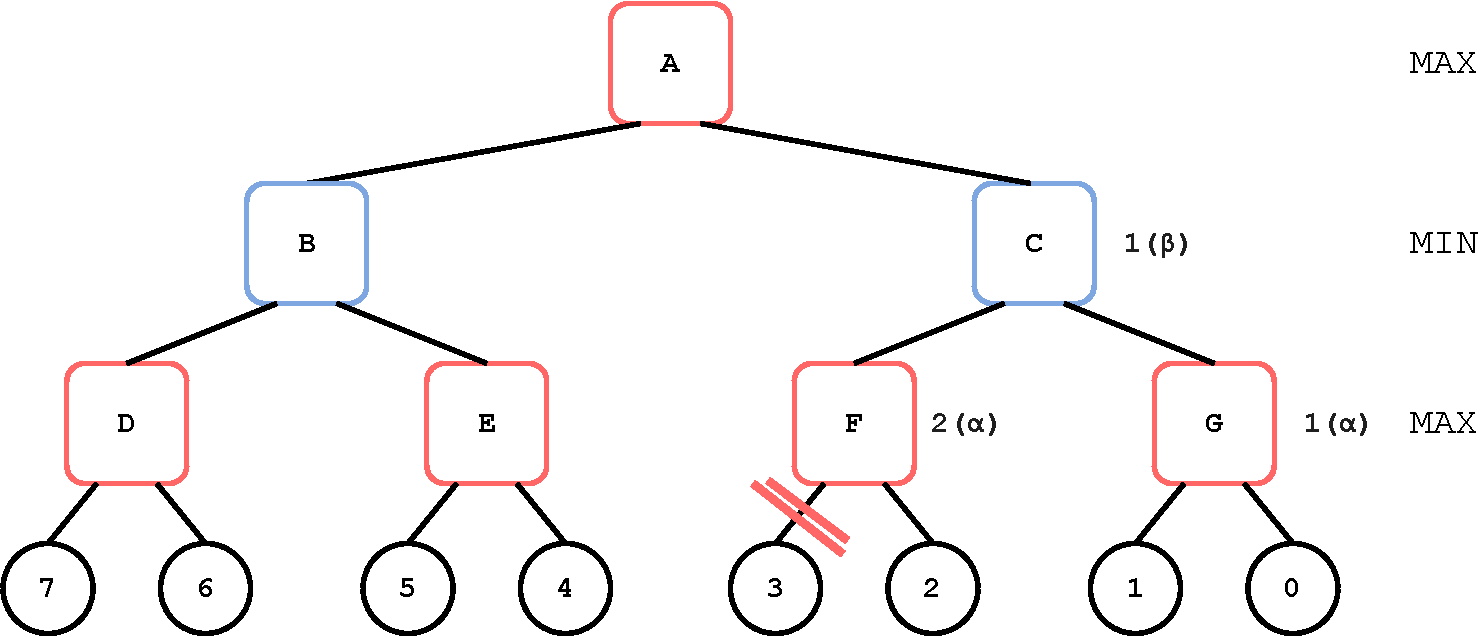
\includegraphics[width=\columnwidth]{../design/assets/alpha_beta_pruning.pdf}
    \caption{Example minimax tree with alpha-beta pruning}
    \label{fig:alpha-beta}
\end{figure}

Since minimax is a depth-first search algorithm, nodes $C$ and $G$ and their $\alpha$ and $\beta$ have already been searched. Next, at node $F$, the current $\alpha$ and $\beta$ are $-\infty$ and 1 respectively, since the $\beta$ is passed down from node $C$. Searching the first leaf node, the $\alpha$ subsequently becomes $\alpha=max(-\infty,2)$. This means that the maximising player at this depth is already guaranteed an evaluation of 2 or greater. Since we know that the minimising player at the depth above is guaranteed a value of 1, there is no point in continuing to search node $F$, a node that is returns a value of 2 or greater. Hence at node $F$, where $\alpha\geq\beta$, the branches are pruned.

Alpha-beta pruning therefore prunes insignificant nodes by maintain an upper bound $\alpha$ and lower bound $\beta$. This is an essential optimization as a simple minimax tree increases exponentially in size with each depth ($O(b^d)$, with branching factor $b$ and $d$ ply depth), and alpha-beta reduces this and the associated computational time considerably.
\\
The pseudocode implementation is shown below:

\begin{algorithm}[H]
\caption{Minimax with alpha-beta pruning pseudocode}
\begin{algorithmic}
    \Function{minimax}{node, depth, $\alpha$, $\beta$, maximisingPlayer}
        \If{$depth = 0$ \textbf{OR} node equals game over}
            \State \Return{\Call{evaluate}{}}
        \EndIf

        \bigskip

        \If{maximisingPlayer}
            \State $value \gets -\infty$
            \For{child of node}
                \State $value \gets \Call{max}{value, \Call{minimax}{child, depth - 1, \alpha, \beta, false}}$
                \If{$value > \beta$}
                    \textbf{break}
                \EndIf
                \State $\alpha \gets \Call{max}{\alpha, value}$
            \EndFor
            \State \Return{$value$}
        \Else
            \State $value \gets +\infty$
            \For{child of node}
                \State $value \gets \Call{min}{value, \Call{minimax}{child, depth - 1, \alpha, \beta, true}}$
                \If{$value < \alpha$}
                    \textbf{break}
                \EndIf
                \State $\beta \gets \Call{min}{\beta, value}$
            \EndFor
            \State \Return{$value$}
        \EndIf
    \EndFunction
\end{algorithmic}
\end{algorithm}

\subsubsection*{Transposition Tables \& Zobrist Hashing}
\label{sec:design-cache}
Transition tables, a memoisation technique, again greatly reduces the number of moves searched. During a brute-force minimax search with a depth greater than 1, the same positions may be searched multiple times, as the same position can be reached from different sequences of moves. A transposition table caches these same positions (transpositions), along with their associated evaluations, meaning commonly reached positions are not unnecessarily re-searched.

Flags and depth are also stored alongside the evaluation. Depth is required as if the current search comes across a cached position with an evaluation calculated at a lower depth than the current search, the evaluation may be inaccurate. Flags are required for dealing with the uncertainty involved with alpha-beta pruning, and can be any of the following three.

\paragraph{Exact} flag is used when a node is fully searched without pruning, and the stored and fetched evaluation is accurate.
\paragraph{Lower} flag is stored when a node receives an evaluation greater than the $\beta$, and is subsequently pruned, meaning that the true evaluation could be higher than the value stored. We are thus storing the $\alpha$ and not an exact value. Thus, when we fetch the cached value, we have to recheck if this value is greater than $\beta$. If so, we return the value and this branch is pruned (fail high); If not, nothing is returned, and the exact evaluation is calculated.
\paragraph{Upper} flag is stored when a node receives an evaluation smaller than the $\alpha$, and is subsequently pruned, meaning that the true evaluation could be lower than the value stored. Similarly, when we fetch the cached value, we have to recheck if this value is lower than $\alpha$. Again, the current branch is pruned if so (fail low), and an exact evaluation is calculated if not.

\bigskip

\noindent The pseudocode implementation for transposition tables is shown below:

\begin{algorithm}[H]
\caption{Minimax with transposition table pseudocode}
\begin{algorithmic}
    \Function{minimax}{node, depth, $\alpha$, $\beta$, maximisingPlayer}
        \State $hash\_key \gets \Call{hash}{node}$
        \State $entry \gets \Call{getentry}{hash\_key}$

        \bigskip

        \If{$entry.hash\_key = hash\_key$ \textbf{AND} $entry.hash\_key \geq depth$}
            \If{$entry.hash\_key = \textbf{EXACT}$}
                \State \Return{$entry.value$}
            \ElsIf{$entry.hash\_key = \textbf{LOWER}$}
                \State $\alpha \gets \Call{max}{\alpha, entry.value}$

            \ElsIf{$entry.hash\_key = \textbf{UPPER}$}
                \State $\beta \gets \Call{min}{\beta, entry.value}$
            \EndIf

            \If{$\alpha\geq\beta$}
                \State \Return{$entry.value$}
            \EndIf
        \EndIf

        \bigskip

        \textit{...normal minimax...}

        \bigskip

        \State $entry.value \gets value$
        \State $entry.depth \gets depth$
        \If{$value \leq \alpha$}
            \State $entry.flag \gets \textbf{UPPER}$
        \ElsIf{$value \geq \beta$}
            \State $entry.flag \gets \textbf{LOWER}$
        \Else
            \State $entry.flag \gets \textbf{EXACT}$
        \EndIf

        \bigskip

        \Return{$value$}
    \EndFunction
\end{algorithmic}
\end{algorithm}

The current board position will be used as the index for a transposition table entry. To convert our board state and bitboards into a valid index, Zobrist hashing may be used. For every square on the chessboard, a random integer is assigned to every piece type (12 in our case, 6 piece type, times 2 for both colours). To initialise a hash, the random integer associated with the piece on a specific square undergoes an XOR operation with the existing hash. The hash is incrementally updated with XOR operations every move, instead of being recalculated from scratch improving computational efficiency. Using XOR operations also allows moves to be reversed, proving useful for the functionality to scroll through previous moves. A Zobrist hash is also a better candidate than FEN strings in checking for threefold-repetition, as they are less intensive to calculate for every move.
\\
The pseudocode implementation for Zobrist hashing is shown below:

\begin{algorithm}[H]
\caption{Zobrist hashing pseudocode}
\begin{algorithmic}
    \item \textit{RANDOMINTS represents a pre-initialised array of random integers for each piece type for each square}

    \bigskip

    \Function{hash\_board}{board}
        \State $hash \gets 0$

        \For{each square on board}
            \If{square is not empty}
                \State $hash \oplus RANDOMINTS[square][$\textit{piece on square}$]$
            \EndIf
        \EndFor

        \State \Return $hash$
    \EndFunction

    \bigskip

    \Function{updatehash}{hash, move}
        \State $hash \oplus RANDOMINTS[$\textit{source square}$][$\textit{piece}$]$
        \State $hash \oplus RANDOMINTS[$\textit{destination square}$][$\textit{piece}$]$

        \If{red to move}
            \State $hash \oplus \textit{hash for red to move}$ \Comment{Hash needed for move colour, as two identical positions are different if the colour to move is different}
        \EndIf

        \State \Return $hash$
    \EndFunction
\end{algorithmic}
\end{algorithm}

\subsubsection*{Iterative Deepening}
\label{sec:design-deepening}
Iterative deepening builds upon the previous alpha-beta and caching improvements. A search is initiated at a depth of one ply, which upon finishing, another starts at depth two, three, and increases until the max depth is reached or time allocated is up. Although this means that more nodes are searched, the improvements come from the fact that the best move (PV-Move) found by a lower depth search, can be used as the first move searched on the next higher depth search. This increases the chance of pruning, reducing the net number of nodes searched, and also provides a 'fallback' move if a higher depth search is interrupted.

\subsection{Board Representation}
\subsubsection*{FEN string}
Forsyth-Edwards Notation (FEN) notation provides all information on a particular position in a chess game. I intend to implement methods parsing and generating FEN strings in my program, in order to load desired starting positions and save games for later play. Deviating from the classic 6-part format, a custom FEN string format will be required for our laser chess game, accommodating its different rules from normal chess.
\\
Our custom format implementation is show by the example below:

\begin{center}
sc3ncfancpb2/2pc7/3Pd7/pa1Pc1rbra1pb1Pd/pb1Pd1RaRb1pa1Pc/6pb3/7Pa2/2PdNaFaNa3Sa r
\end{center}

\noindent Our FEN string format contains two parts, denoted by the space between them:

\begin{itemize}
\item Part 1: Describes the location of each piece. The construction of this part is defined by the following rules:
\begin{itemize}
\item The board is read from top-left to bottom-right, row by row
\item A number represents the number of empty squares before the next piece
\item A capital letter represents a blue piece, and a lowercase letter represents a red piece
\item The letters $F$, $R$, $P$, $N$, $S$ stand for the pieces Pharaoh, Scarab, Pyramid, Anubis and Sphinx respectively
\item Each piece letter is followed by the lowercase letters $a$, $b$, $c$ or $d$, representing a 0°, 90°, 180° and 270° degree rotation respectively
\end{itemize}
\item Part 2: States the active colour, $b$ means blue to move, $r$ means red to move
\end{itemize}

Having inputted the desired FEN string board configuration in the config menu, the bitboards for each piece will be initialised with the following functions:

\begin{algorithm}[H]
\caption{FEN string pseudocode}
\label{alg:fen-string}
\begin{algorithmic}
    \Function{parse\_fen\_string}{fen\_string, board}
        \State $part\_1, part\_2 \gets \Call{split}{fen\_string}$

        \State$rank \gets 8$
        \State$file \gets 0$

        \bigskip

        \For{character in part\_1}
            \State$square \gets rank \times 8 + file$

            \If{character is alphabetic}
                \If{character is lower}
                    \State $board.bitboards[red][character] \quad | \quad 1 << character$
                \Else
                    \State $board.bitboards[blue][character] \quad | \quad 1 << character$
                \EndIf
            \ElsIf{character is numeric}
                \State $file \gets file + character$
            \ElsIf{$character is /$}
                \State $rank \gets rank - 1$
                \State $file \gets file + 1$
            \Else
                \State $file \gets file + 1$
            \EndIf

        \bigskip

        \If{part\_2 is b}
            \State $board.active\_colour \gets b$
        \Else
            \State $board.active\_colour \gets r$
        \EndIf
        \EndFor
    \EndFunction
\end{algorithmic}
\end{algorithm}

The function first processes every piece and corresponding square in the FEN string, modifying each piece bitboard using a bitwise OR operator, with a 1 shifted over to the correctly occupied square using a Left-Shift operator. For the second part, the active colour property of the board class is initialised to the correct player.

\subsubsection*{Bitboards}
\label{sec:design-bitboards}
Bitboards are an array of bits representing a position or state of a board game. Multiple bitboards are used with each representing a different property of the game (e.g. scarab position and scarab rotation), and can be masked together or transformed to answer queries about positions. Bitboards offer an efficient board representation, its performance primarily arising from the speed of parallel bitwise operations used to transform bitboards.
To map each board square to a bit in each number, we will assign each square from left to right, with the least significant bit (LSB) assigned to the bottom-left square (A1), and the most significant bit (MSB) to the top-right square (J8).

\begin{figure}[H]
    \centering
    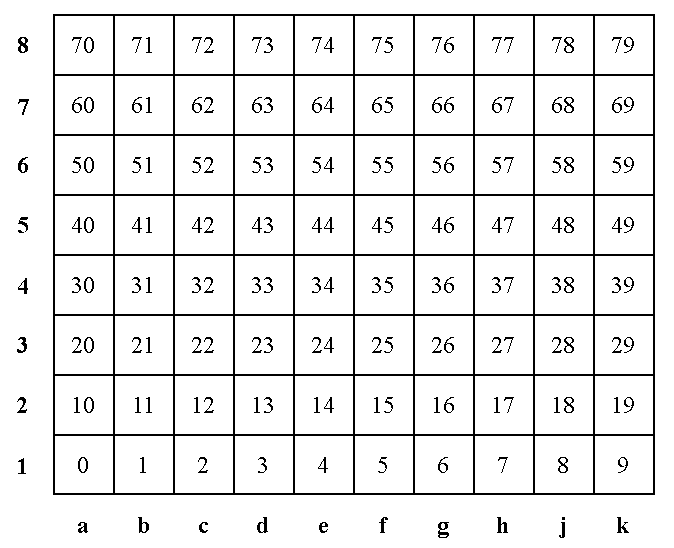
\includegraphics[width=0.6\columnwidth]{../design/assets/bitboard_indexes.pdf}
    \caption{Square to bit position mapping}
    \label{fig:bitboard-indexes}
\end{figure}

Firstly, we need to initialise each bitboard and place 1s in the correct squares occupied by pieces. This is achieved whilst parsing the FEN-string, as shown in Algorithm \ref{alg:fen-string}.
Secondly, we should implement an approach to calculate possible moves using our computed bitboards. We can begin by producing a bitboard containing the locations of all pieces, achieved through combining every piece bitboard with bitwise OR operations:

\begin{center}
all\_pieces\_bitboard = white\_pharaoh\_bitboard $\vert$  black\_pharaoh\_bitboard $\vert$ white\_scarab\_bitboard ...
\end{center}

Now, we can utilize this aggregated bitboard to calculate possible positional moves for each piece.
For each piece, we can shift the entire bitboard to an adjacent target square (since every piece can only move one adjacent square per turn), and perform a bitwise AND operator with the bitboard containing all pieces, to determine if the target square is already occupied by an existing piece. For example, if we want to compute if the square to the left of our selected piece is available to move to, we will first shift every bit right (as the lowest square index is the LSB on the right, see diagram above), as demonstrated in the following 5x5 example:

\begin{figure}[H]
    \centering
    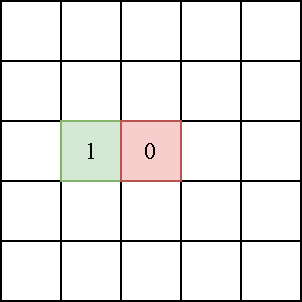
\includegraphics[width=0.4\columnwidth]{../design/assets/bitboard_shifted.pdf}
    \caption{shifted\_bitboard = piece\_bitboard $>>$ 1}
    \label{fig:bitboard-shifted}
\end{figure}

Where green represents the target square shifted into, and orange where the piece used to be. We can then perform a bitwise AND operation with the complement of the all pieces bitboard, where a square with a result of 1 represents an available target square to move to.

\begin{center}
available\_squares\_right = (piece\_bitboard $>>$ 1) \& $\sim$ all\_pieces\_bitboard
\end{center}

However, if the piece is on the leftmost A file, and is shifted to the right, it will be teleported onto the J file on the rank below, which is not a valid move. To prevent these erroneous moves for pieces on the edge of the board, we can utilise an A file mask to mask away any valid moves, as demonstrated below:

\begin{figure}[H]
    \centering
    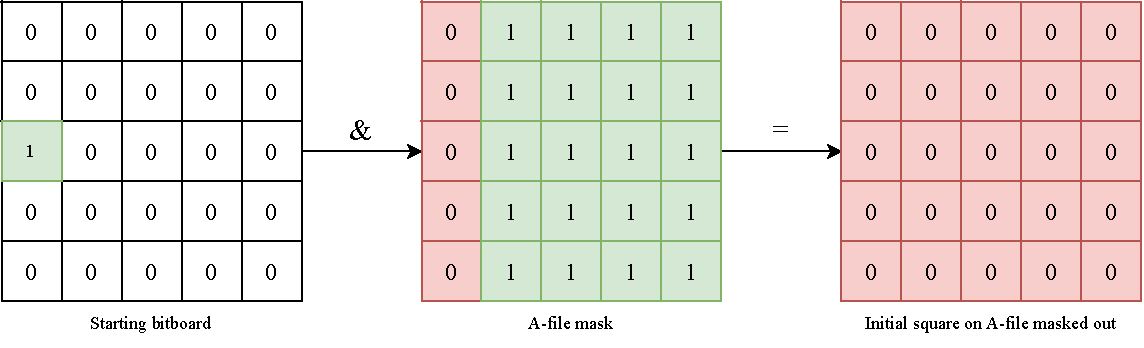
\includegraphics[width=\columnwidth]{../design/assets/bitboard_masked.pdf}
    \caption{A-file mask example}
    \label{fig:bitboard-masked}
\end{figure}

This approach uses the logic that a piece on the A file can never move to a square on the left. Therefore, when calculating if a piece can move to a square on the left, we apply a bitwise AND operator with a mask where every square on the A file is 0; If a piece was on the A file, it will become 0, leaving no possible target squares to move to. The same approach can be mirrored for the far-right J file.

In theory, we do not need to implement the same solution for clipping in regard to ranks, as they are removed automatically by overflow or underflow when shifting bits too far.
Our final function to calculate valid moves combines all the logic above: Shifting the selected piece in all 9 adjacent directions by their corresponding bits, masking away pieces trying to move into the edge of the board, combining them with a bitwise OR operator, and finally masking it with the all pieces bitboard to detect which squares are not currently occupied:

\begin{algorithm}[H]
\caption{Finding valid moves pseudocode}
\label{alg:valid-moves}
\begin{algorithmic}
    \Function{find\_valid\_moves}{selected\_square}
    \State $masked\_a\_square \gets selected\_square$ \&  $A\_FILE\_MASK$
    \State $masked\_j\_square \gets selected\_square$ \& $J\_FILE\_MASK$

    \bigskip

    \State $top\_left \gets masked\_a\_square << 9$

	\State $top\_left \gets masked\_a\_square << 9$
	\State $top\_middle \gets selected\_square << 10$
	\State $top\_right \gets masked\_ << 11$
	\State $middle\_right \gets masked\_ << 1$

	\State $bottom\_right \gets masked\_ >> 9$
	\State $bottom\_middle \gets selected\_square >> 10$
	\State $bottom\_left \gets masked\_a\_square >> 11$
	\State $middle\_left \gets masked\_a\_square >> 1$

    \bigskip

    \State $possible\_moves = top\_left$ $\vert$ $top\_middle$ $\vert$ $top\_right$ $\vert$ $middle\_right$ $\vert$ $bottom\_right$ $\vert$ $bottom\_middle$ $\vert$ $bottom\_left$ $\vert$ $middle\_left$

    \State $valid\_moves = possible\_moves$ \& $\sim ALL\_PIECES\_BITBOARD$

    \bigskip

    \State \Return $valid\_moves$
    \EndFunction
\end{algorithmic}
\end{algorithm}

\subsection{Evaluation Function}
\label{sec:design-evaluation}
The evaluation function is a heuristic algorithm to determine the relative value of a position. It outputs a real number corresponding to the advantage given to a player if reaching the analysed position, usually at a leaf node in the minimax tree. The evaluation function therefore provides the values on which minimax works on to compute an optimal move.

In the majority of evaluation functions, the most significant factor determining the evaluation is the material balance, or summation of values of the pieces. The hand-crafted evaluation function is then optimised by tuning various other positional weighted terms, such as board control and king safety.

\subsubsection*{Material Value}
Since laser chess is not widely documented, I have assigned relative strength values to each piece according to my experience playing the game:

\begin{itemize}
\item Pharaoh - $\infty$
\item Scarab - 200
\item Anubis - 110
\item Pyramid - 100
\end{itemize}

To find the number of pieces, we can iterate through the piece bitboard with the following popcount function:

\begin{algorithm}[H]
\caption{Popcount pseudocode}
\label{alg:popcount}
\begin{algorithmic}
    \Function{popcount}{bitboard}
    \State $count \gets 0$

    \While{bitboard}
        \State $count \gets count + 1$
        \State $bitboard \gets bitboard \& (bitboard - 1)$
    \EndWhile

    \State \Return $count$
    \EndFunction
\end{algorithmic}
\end{algorithm}

Algorithm \ref{alg:popcount} continually resets the left-most 1 bit, incrementing a counter for each loop. Once the number of pieces has been established, we multiply this number by the piece value. Repeating this for every piece type, we can thus obtain a value for the total piece value on the board.

\subsubsection*{Piece-Square Tables}
A piece in normal chess can differ in strength based on what square it is occupying. For example, a knight near the centre of the board, controlling many squares, is stronger than a knight on the rim. Similarly, we can implement positional value for Laser Chess through Piece-Square Tables. PSQTs are one-dimensional arrays, with each item representing a value for a piece type on that specific square, encoding both material value and positional simultaneously. Each array will consist of 80 base values representing the piece’s material value, with a bonus or penalty added on top for the location of the piece on each square. For example, the following PSQT is for the pharaoh piece type on an example 5x5 board:

\begin{figure}[H]
    \centering
    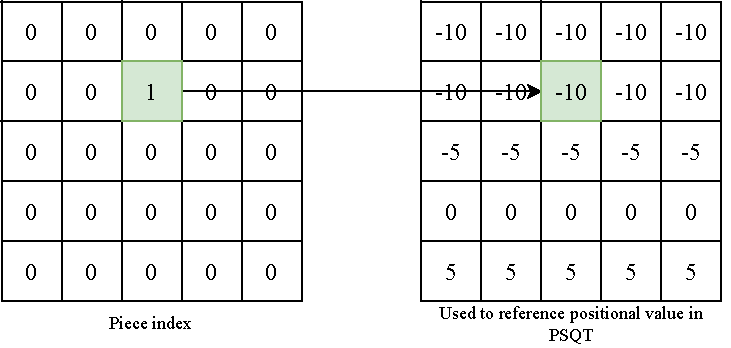
\includegraphics[width=0.8\columnwidth]{../design/assets/psqt.pdf}
    \caption{PSQT showing the bonus position value gained for the square occupied by a pharaoh}
    \label{fig:psqt}
\end{figure}

For asymmetrical PSQTs, we would ideally like to label the board identically from both player’s point of views. Although the PSQTs are displayed from the blue player's perspective (blue pharaoh at the bottom of the board), it uses indexes from the red player's perspective, as arrays and lists are defined with index 0 being at the topleft of the board. We would like to flip the PSQTs to be reused with blue indexes, so that a generic algorithm can be used to sum up and calculate the total positional values for both players.

To utilise a PSQT for blue pieces, a special ‘FLIP’ table can be implemented:

\begin{figure}[H]
    \centering
    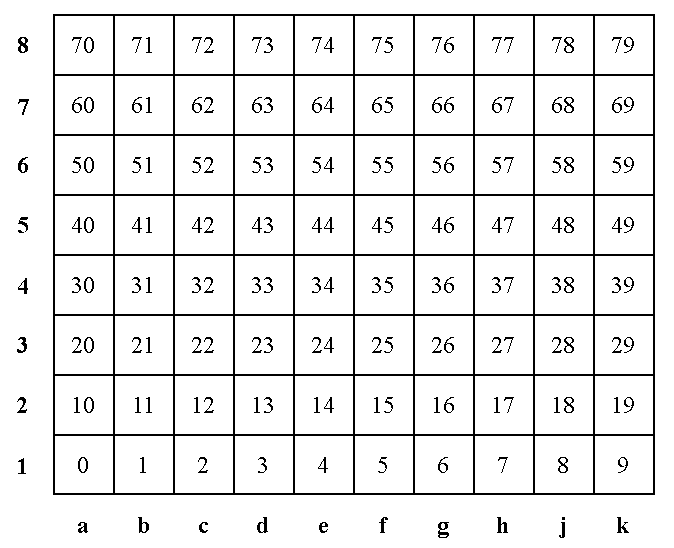
\includegraphics[width=0.6\columnwidth]{../design/assets/bitboard_indexes.pdf}
    \caption{FLIP table used to map a blue piece index to the red player's perspective}
    \label{fig:flip-table}
\end{figure}

The FLIP table is just an array of indexes, mapping every blue player’s index onto the corresponding red index. The following expression utilises the FLIP table to retrieve a blue player’s value from the red player’s PSQT:

\begin{center}
blue\_psqt\_value = PHARAOH\_PSQT[FLIP[square]]
\end{center}

The following function retrieves an array of bitboards representing piece positions from the board class, then sums up all the values of these pieces for both players, referencing the corresponding PSQT:

\begin{algorithm}[H]
\caption{Calculating positional value pseudocode}
\begin{algorithmic}
    \Function{calculate\_positional\_value}{bitboards, colour}
    \State $positional\_score \gets 0$

    \ForAll{pieces}
        \For {square in bitboards[piece]}
            \If{$square = 1$}
                \If{$colour$ \textbf{is} $blue$}
                    \State $positional\_score \gets positional\_score + PSQT[piece][square]$
                \Else
                    \State $positional\_score \gets positional\_score + PSQT[piece][FLIP[square]]$
                \EndIf
            \EndIf
        \EndFor
    \EndFor

    \State \Return $positional\_score$
    \EndFunction
\end{algorithmic}
\end{algorithm}

\subsubsection*{Using valid squares}
Using Algorithm \ref{alg:valid-moves} for finding valid moves, we can implement two more improvements for our evaluation function: Mobility and King Safety.

\paragraph{Mobility} is the number of legal moves a player has for a given position. This is advantageous in most cases, with a positive correlation between mobility and the strength of a position. To implement this, we simply loop over all pieces of the active colour, and sum up the number of valid moves obtained from the previous algorithm.

\paragraph{King safety} (Pharaoh safety) describes the level of protection of the pharaoh, being the piece that determines a win or loss. In normal chess, this would usually be achieved by castling, or protection via position or with other pieces. Similarly, since the only way to lose in Laser Chess is via a laser, having pieces surrounding the pharaoh, either to reflect the laser or to be sacrificed, is a sensible tactic and improves king safety. Thus, a value for king safety can be achieved by finding the number of valid moves a pharaoh can make, and subtracting them from the maximum possible of moves (8) to find the number of surrounding pieces.

\subsection{Shadow Mapping}
\label{sec:design-shadow}
Following the client's requirement for engaging visuals, I have decided to implement shadow mapping for my program, especially as lasers are the main focus of the game. Shadow mapping is a technique used to create graphical hard shadows, with the use of a depth buffer map. I have chosen to implement shadow mapping, instead of alternative lighting techniques such as ray casting and ray marching, as its efficiency is more suitable for real-time usage, and results are visually decent enough for my purposes.
\\
For typical 3D shadow mapping, the standard approach is as follows:

\begin{enumerate}
\item Render the scene from the light's point of view
\item Extract a depth buffer texture from the render
\item Compare the distance of a pixel from the light to the value stored in the depth texture
\item If greater, there must be an obstacle in the way reducing the depth map value, therefore that pixel must be in shadow
\end{enumerate}

\noindent To implement shadow casting for my 2D game, I have modified some steps and arrived on the final following workflow:

\begin{enumerate}
\item Render the scene with only occluding objects shown
\item Crop texture to align the centre to the light position
\item To create a 1D depth map, transform Cartesian to polar coordinates, and increase the distance from the origin until a collision with an occluding object
\item Using polar coordinates for the real texture, compare the z-depth to the corresponding value from the depth map
\item Additively blend the light colour if z-depth is less than the depth map value
\end{enumerate}

\begin{figure}[H]
    \centering
    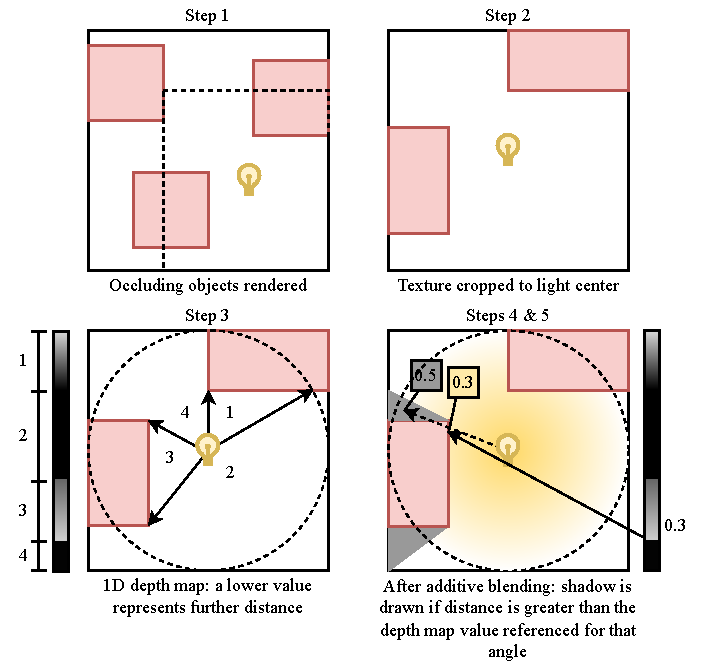
\includegraphics[width=\columnwidth]{../design/assets/shadow_mapping.pdf}
    \caption{Workflow for 2D shadow mapping}
    \label{fig:shadow-mapping}
\end{figure}

Our method requires a coordinate transformation from Cartesian to polar, and vice versa. Polar to Cartesian transformation can be achieved with trigonometry, forming a right-angled triangle in the centre and using the following two equations:
\begin{align*}
x &= r\cos(\theta)\\
y &= r\sin(\theta)
\end{align*}

Cartesian to polar can also similarly be achieved with the right-angled triangle, finding the radius with the Pythagorean theorem, and the angle with arctan. However, since the range of the arctan function is only a half-circle ($\frac{\pi}{2} < \theta < \frac{\pi}{2}$), we will have to use the atan2 function, which accounts for the negative quadrants, or the following:

\begin{equation*}
\theta = 2\arctan\left(\frac{r - x}{y}\right)
\end{equation*}

There are several disadvantages to shadow mapping. The relevant ones for us are Aliasing and Shadow Acne:

\paragraph{Aliasing} occurs when the texture size for the depth map is smaller than the light map, causing shadows to be scaled up and rendered with jagged edges.

\paragraph{Shadow Acne} occurs when the depth from the depth map is so close to the light map value, that precision errors cause unnecessary shadows to be rendered.

\bigskip

\noindent These problems can be mitigated by increasing the size of the shadow map size. However, due to memory and hardware constraints, I will have to find a compromised resolution to balance both artifacting and acuity.

\subsubsection*{Soft Shadows}
To approach above is used only for calculating hard shadows. However, in real-life scenarios, lights are not modelled as a single particle, but instead emitted from a wide light source. This creates an umbra and penumbra, resulting in soft shadows.

To emulate this in our game, we could calculate penumbra values with various methods, however, due to hardware constraints and simplicity again, I have chosen to use the following simpler method:

\begin{enumerate}
\item Sample the depth map multiple times, from various differing angles
\item Sum the results using a normal distribution
\item Blur the final result proportional to the length from the centre
\end{enumerate}

\begin{figure}[H]
    \centering
    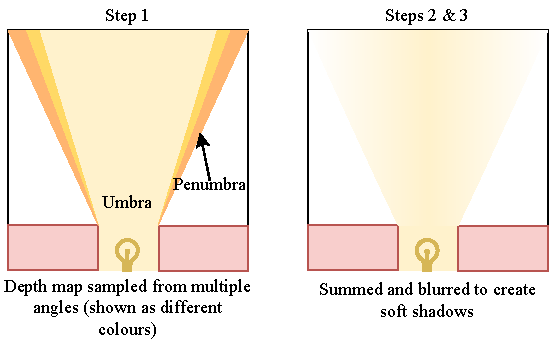
\includegraphics[width=0.8\columnwidth]{../design/assets/soft_shadows.pdf}
    \caption{Workflow for 2D soft shadows}
    \label{fig:soft-shadows}
\end{figure}

This method progressively blurs the shadow as the distance from the main shadow (umbra) increases, which results in a convincing estimation while being less computationally intensive.

\subsection{Multithreading}
\label{sec:design-multithreading}
In order to fulfil Objective \ref{itm:responsive-objective} of a responsive GUI, I will have to employ multi-threading. Since python runs on a single thread natively, code is executed serially, meaning that a time-consuming function such as minimax will prevent the running of another GUI-drawing function until it is finished, hence freezing the program. To overcome this, multi-threading can execute both functions in parallel on different threads, meaning the GUI-drawing thread can run while minimax is being computed, and stay responsive. To pass data between threads, since memory is shared between threads, arrays and queues can be used to store results from threads. The following flowchart shows my chosen approach to keep the GUI responsive while minimax is being computed:

\begin{figure}[H]
    \centering
    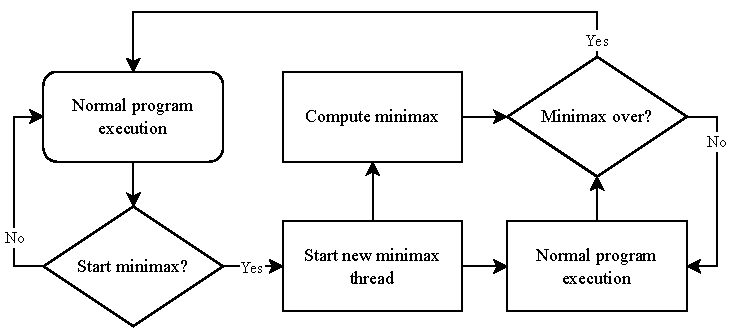
\includegraphics[width=\columnwidth]{../design/assets/multi_threading.pdf}
    \caption{Multi-threading for minimax}
    \label{fig:multi-threading}
\end{figure}

\section{Data Structures}
\subsection{Database}
To achieve Objective \ref{itm:save-games} and stores previous games, I have opted to use a relational database. Choosing between different relational database, I have decided to use SQLite, since it does not require additional server software, has good performance with low memory requirements, and adequate for my use cases, with others such as Postgres being overkill.

\subsubsection*{DDL}
\label{sec:design-ddl}
Only a single entity will be required for my program, a table to store games. The table schema will be defined as follows:

\begin{longtable}[c]{l|l|l|l}
    \multicolumn{4}{l}{\textbf{Table: games}}\\
    \toprule
    \textbf{Field} & \textbf{Key} & \textbf{Data Type} & \textbf{Validation}\\
    \midrule
    \endfirsthead
    \endhead

    game\_id & Primary & INT & NOT NULL\\
    winner &  & INT & \\
    cpu\_depth &  & INT & \\
    number\_of\_moves &  & INT & NOT NULL\\
    cpu\_enabled &  & BOOL & NOT NULL\\
    moves &  & TEXT & NOT NULL\\
    initial\_board\_configuration &  & TEXT & NOT NULL\\
    time &  & FLOAT & \\
    created\_dt &  & TIMESTAMP & NOT NULL\\

    \bottomrule

\caption{Data table scheme for \textit{games} table}
\label{tab:games-schema}
\end{longtable}

All fields are either generated or retrieved from the board class, except the moves attribute, which will need to be encoded into a suitable data type such as a string. All attributes are also independent of each other\footnote{There is a case to be made for \textit{moves} and \textit{number\_of\_moves}, however I have included \textit{number\_of\_moves} to save the computational effort of parsing the moves for every game just to display it on the browser preview section.}, and so the table therefore adheres to the third normal form.

To create the entity, a \lstinline[language=sqlite]{CREATE} statement like the following can be used:

\begin{lstlisting}[language=sqlite, frame=lines]
    CREATE TABLE games(
        id INTEGER PRIMARY KEY,
        winner INTEGER,
        cpu_depth INTEGER,
        time real NOT NULL,
        moves TEXT NOT NULL,
        cpu_enabled INTEGER NOT NULL,
        created_dt TIMESTAMP NOT NULL,
        number_of_moves INTEGER NOT NULL,
        initial_fen_string TEXT NOT NULL,
    )
\end{lstlisting}

\noindent Removing an entity can also be done similarly:

\begin{lstlisting}[language=sqlite, frame=lines]
    DROP TABLE games
\end{lstlisting}

Migrations are a version control system to track incremental changes to the schema of a database. Since there is no popular SQL Python-binding libraries that support migrations, I will just be using a manual solution of creating python files that represent a change in my schema, defining functions that make use of SQL \lstinline[language=sqlite]{ALTER} statements. This allows me to keep track of any changes, and rollback to a previous schema.

\subsubsection*{DML}
\label{sec:design-dml}
To insert a new game entry into the table, an \lstinline[language=sqlite]{INSERT} statement can be used with the provided array, where the appropriate arguments are bound to the correct attribute via \lstinline[language=Python]{?} placeholders when run.

\begin{lstlisting}[language=sqlite, frame=lines]
    INSERT INTO games (
        cpu_enabled,
        cpu_depth,
        winner,
        time,
        number_of_moves,
        moves,
        initial_fen_string,
        created_dt
    )
    VALUES (?, ?, ?, ?, ?, ?, ?, ?)
\end{lstlisting}

Moreover, we will need to fetch the number of total game entries in the table to be displayed to the user. To do this, the aggregate function \lstinline[language=sqlite]{COUNT} can be used, which is supported by all SQL databases.

\begin{lstlisting}[language=sqlite, frame=lines]
    SELECT COUNT(*) FROM games
\end{lstlisting}

\subsubsection*{Pagination}
When there are a large number of entries in the table, it would be appropriate to display all the games to the user in a paginated form, where they can scroll between different pages and groups of games. There are multiple methods to paginate data, such as using \lstinline[language=sqlite]{LIMIT} and \lstinline[language=sqlite]{OFFSET} clauses, or cursor-based pagination, but I have opted to use the \lstinline[language=sqlite]{ROW_NUMBER()} function.

\lstinline[language=sqlite]{ROW_NUMBER()} is a window function that assigns a sequential integer to a query's result set. If I were to query the entire table, each row would be assigned an integer that could be used to check if the row is in the bounds for the current page, and therefore be displayed. Moreover, the use of an \lstinline[language=sqlite]{ORDER BY} clause enables sorting of the output rows, allowing the user to choose what order the games are presented in based on an attribute such as number of moves. A \lstinline[language=sqlite]{PARTITION BY} clause will also be used to group the results base on an attribute such as winner prior to sorting, if the user wants to search for games based on multiple criteria with greater ease.

The start row and end row will be passed as parameters to the placeholders in the SQL statement, calculated by multiplying the page number by the number of games per page.

\begin{lstlisting}[language=sqlite, frame=lines]
    SELECT * FROM
        (SELECT ROW_NUMBER() OVER (
            PARTITION BY (*@\textit{attribute1}@*)
            ORDER BY (*@\textit{attribute2}@*) ASC
        ) AS row_num, * FROM games)
    WHERE row_num >= ? AND row_num <= ?
\end{lstlisting}

\subsubsection*{Security}
Security measures such as database file permissions and encryption are common for a SQL database. However, since SQLite is a serverless database, and my program runs without any need for an internet connection, the risk of vulnerabilities is greatly reduced. Additionally, the game data stored on my database is frankly inconsequential, so going to great lengths to protect it wouldn't be to best use of my time. Nevertheless, my SQL Python-binding does support the user of placeholders for parameters, thereby addressing the risk of SQL injection attacks.

\subsection{Linked Lists}
\label{sec:linked-lists}
\begin{figure}[H]
    \centering
    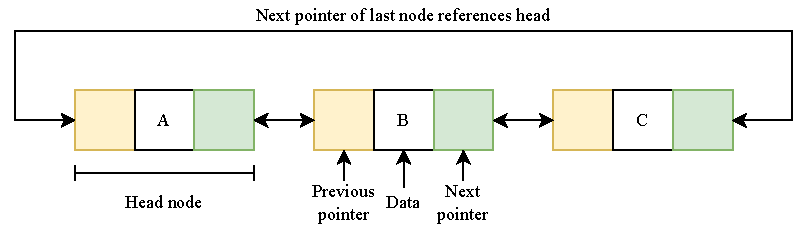
\includegraphics[width=\columnwidth]{../design/assets/linked_list.pdf}
    \caption{Structure of a circular doubly-linked list}
    \label{fig:linked-list}
\end{figure}

Another data structure I intend to implement is linked lists. This will be integrated into widgets such as the carousel or multiple icon button widget, since these will contain a variable number of items, and where $O(1)$ random access is not a priority. Since moving back and forth between nodes is a must for a carousel widget, the linked list will be doubly-linked, with each node containing to its previous and next node. The list will also need to loop, with the next pointer of the last node pointing back to the first node, making it a circular linked list, as demonstrated in Figure \ref{fig:linked-list}.

The following pseudocode outlines the basic functionality of the linked list:

\begin{algorithm}[H]
\caption{Circular doubly linked list pseudocode}
\begin{algorithmic}
    \Function{insert\_at\_front}{node}
        \If{head is none}
            \State $head \gets node$
            \State $node.next \gets node.previous \gets head$
        \Else
            \State $node.next \gets head$
            \State $node.previous \gets head.previous$
            \State $head.previous.next \gets node$
            \State $head.previous \gets node$

            \bigskip

            \State $head \gets node$
        \EndIf
    \EndFunction

    \bigskip

    \State \Require $\Call{len}{list} > 0$
    \Function{data\_in\_list}{data}

        \State $current\_node \gets head.next$
        \While{$current\_node \neq head$}
            \If{$current\_node.data = data$}
                \State \Return \textbf{True}
            \EndIf
            \State $current\_node \gets current\_node.next$
        \EndWhile

        \State \Return \textbf{False}
    \EndFunction

    \bigskip

    \State \Require Data in list
    \Function{remove}{data}
        \State $current\_node \gets head$
        \While{$current\_node.data \neq data$}
            \State $current\_node \gets current\_node.next$
        \EndWhile

        \bigskip

        \State $current\_node.previous.next \gets current\_node.next$
        \State $current\_node.next.previous \gets current\_node.previous$

        \bigskip

        \State \textbf{delete} $current\_node$
    \EndFunction
\end{algorithmic}
\end{algorithm}

\subsection{Stack}
\label{sec:design-stack}
Being a data structure with LIFO ordering, a stack is used for handling moves in the review screen. Starting with full stack of moves, every move undone pops an element off the stack to be processed. This move is then pushed onto a second stack. Therefore, cycling between moves requires pushing and popping between the two stacks, as shown in Figure \ref{fig:stack-diagram}. The same functionality can be achieved using a queue, but I have chosen to use two stacks as it is simpler to implement, as being able to quickly check the number of items in each will come in handy.

\begin{figure}[H]
    \centering
    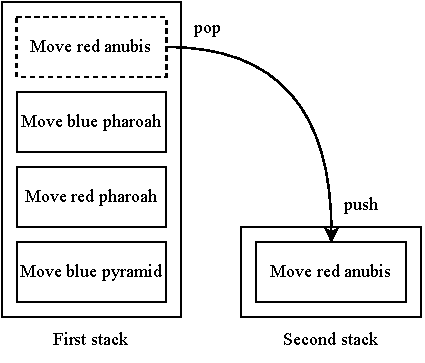
\includegraphics[width=0.6\columnwidth]{../design/assets/stack.pdf}
    \caption{\textit{Move red anubis} is undone and pushed onto the second stack}
    \label{fig:stack-diagram}
\end{figure}

\section{Classes}
I will be using an Object-Oriented Programming (OOP) paradigm for my program. OOP reduces repetition of code, as inheritance can be used to abstract repetitive code into a base class, as show in my widgets implementation. Testing and debugging classes will make my workflow more efficient. This section documents the base classes I am going to implement in my program.

\subsubsection*{State}
Since there will be multiple screens in my program as demonstrated in Figure \ref{fig:program-overview-flowchart}, the State base class will be used to handle the logic for each screen. For each screen, void functions will be inherited and overwritten, each containing their own logic for that specific screen. For example, all screens will call the startup function in Table \ref{tab:state-methods} to initialise variables needed for that screen. This polymorphism approach allows me to use another Control class to enable easy switching between screens, without worrying about the internal logic of that screen. Virtual methods also allow methods such as \lstinline[language=Python]{draw} to be abstracted to the State superclass, reducing code in the inherited subclasses, while allowing them to override the methods and add their own logic.

\begin{longtable}[c]{l|l}
    \toprule
    \textbf{Method Name} & \textbf{Description}\\
    \midrule
    \endfirsthead
    \endhead

    startup & Initialise variables and functions when state set as displayed screen\\
    cleanup & Cleanup any variables and functions when state removed from screen\\
    draw & Draw to display\\
    update & Update any variables for every game tick\\
    handle\_resize & Scale GUI when window resized\\
    get\_event & Receive pygame events as argument and process them\\

    \bottomrule

\caption{Methods for State class}
\label{tab:state-methods}
\end{longtable}

\subsubsection*{Widget}
\label{sec:design-widgets}
I will be implementing my own widget system for creating the game GUI. This allows me to fully customise all graphical elements on the screen, and also create a resizing system that adheres to Objective \ref{itm:responsive-objective}. The default Pygame rescaling options also simply resize elements without accounting for aspect ratios or resolution, and I could not find a library that suits my needs. Having a bespoke GUI implementation also justifies my use of Pygame over other Python frameworks.

I will be utilising the Pygame sprite system for my GUI. All GUI widgets will be subclasses inheriting from the base Widget class, which itself is a subclass of the Pygame sprite class.
Since Pygame sprites are drawn via a \lstinline{SpriteGroup} class, I will also have to create a custom subclass inheriting that as well. As with the State class, polymorphism will allow the \lstinline{SpriteGroup} class to render all widgets regardless of their functionality. Each widget will override their base methods, especially the draw (set\_image) method, for their own needs. Additionally, I will use getter and setter methods, used with the \lstinline[language=Python]{@property} decorator in python, to compute attributes mainly used for resizing widgets. This allows me to expose common variables, and to reduce code repetition.

\begin{longtable}[c]{l|l}
    \toprule
    \textbf{Method Name} & \textbf{Description}\\
    \midrule
    \endfirsthead
    \endhead

    set\_image & Render widget to internal image attribute for Pygame sprite class\\
    set\_geometry & Set position and size of image\\
    set\_screen\_size & Set screen size for resizing purposes\\
    get\_event & Receives Pygame events and processes them\\
    screen\_size* & Returns screen size in pixels\\
    position* & Returns topleft of widget rect\\
    size* & Returns size of widget in pixels\\
    margin* & Returns distance between border and actual widget image\\
    border\_width* & Returns border width\\
    border\_radius* & Returns border radius for rounded corners\\
    font\_size* & Returns font size for text-based widgets\\

    \midrule

    \multicolumn{2}{l}{* represents getter method / property}\\

    \bottomrule

\caption{Methods for Widget class}
\label{tab:widget-methods}
\end{longtable}

I will also employ multiple inheritance to combine different base class functionalities together. For example, I will create a pressable base class, designed to be subclassed along with the widget class. This will provide attributes and methods for widgets that support clicking and dragging. Following Python's Method Resolution Order (MRO), additional base classes should be referenced first, having priority over the base Widget class.

\begin{longtable}[c]{l|l}
    \toprule
    \textbf{Method Name} & \textbf{Description}\\
    \midrule
    \endfirsthead
    \textbf{Method Name} & \textbf{Description}\\
    \midrule
    \endhead

    get\_event & Receives Pygame events and sets current state accordingly\\
    set\_state & Sets current Pressable state, called by \lstinline[language=Python]{get_event}\\
    set\_colours & Set fill colour according to widget Pressable state\\
    current\_state* & Returns current Pressable state (e.g. hovered, pressed etc.)\\

    \midrule

    \multicolumn{2}{l}{* represents getter method / property}\\

    \bottomrule

\caption{Methods for example Pressable class}
\label{tab:pressable-methods}
\end{longtable}

\subsubsection*{Game}
\label{sec:design-mvc}
For my game screen, I will be utilising the Model-View-Controller architectural pattern (MVC). MVC defines three interconnected parts, the model processing information, the view showing the information, and the controlling receiving user inputs and connecting the two. This will allow me to decompose the development process into individual parts for the game logic, graphics and user input, speeding up the development process and making testing easier. It also allows me to implement multiple views, for the pause and win screens as well. For MVC, I will have to implement a game model class, a game controller class, and three classes for each view (game, pause, win). Using aggregation, these will be initially connected and handled by the game state class. For the following methods, I have only showed those pertinent to the MVC pattern:

\begin{longtable}[c]{l|p{0.75\columnwidth}}
    \toprule
    \textbf{Method Name} & \textbf{Description}\\
    \midrule
    \endfirsthead
    \endhead

    get\_event & Receives Pygame events and passes them onto the correct part's event handler\\
    handle\_game\_event & Receives events and notifies the game model and game view\\
    handle\_pause\_event & Receives events and notifies the pause view\\
    handle\_win\_event & Receives events and notifies the win view\\
    ... & ...\\

    \bottomrule

\caption{Methods for Controller class}
\label{tab:controller-methods}
\end{longtable}

\begin{longtable}[c]{l|p{0.75\columnwidth}}
    \toprule
    \textbf{Method Name} & \textbf{Description}\\
    \midrule
    \endfirsthead
    \endhead

    process\_model\_event & Receives events from the model and calls the relevant method to display that information\\
    convert\_mouse\_pos & Sends controller class information of widget under mouse\\
    draw & Draw information to display \\
    handle\_resize & Scale GUI when window resized\\
    ... & ...\\

    \bottomrule

\caption{Methods for View class}
\label{tab:view-methods}
\end{longtable}

\begin{longtable}[c]{l|p{0.75\columnwidth}}
    \toprule
    \textbf{Method Name} & \textbf{Description}\\
    \midrule
    \endfirsthead
    \textbf{Method Name} & \textbf{Description}\\
    \midrule
    \endhead

    register\_listener & Subscribes method on view instance to an event type, so that the method receives and processes that event every time \lstinline[language=Python]{alert_listener} is called\\
    alert\_listener & Sends event to all subscribed instances\\
    toggle\_win & Sends event for win view\\
    toggle\_pause & Sends event for pause view\\
    ... & ...\\

    \bottomrule

\caption{Methods for Model class}
\label{tab:model-methods}
\end{longtable}

\subsubsection*{Shaders}
To use ModernGL with Pygame, I have created classes for each fragment shader, controlled by a main shader manager class. The fragment shader classes will rely on composition: The shader manager creates the fragment shader class; Every fragment shader class takes their shader manager parent instance as an argument, and runs methods on it to produce the final output.

\subsection{Class Diagram}
\begin{figure}[H]
    \centering
    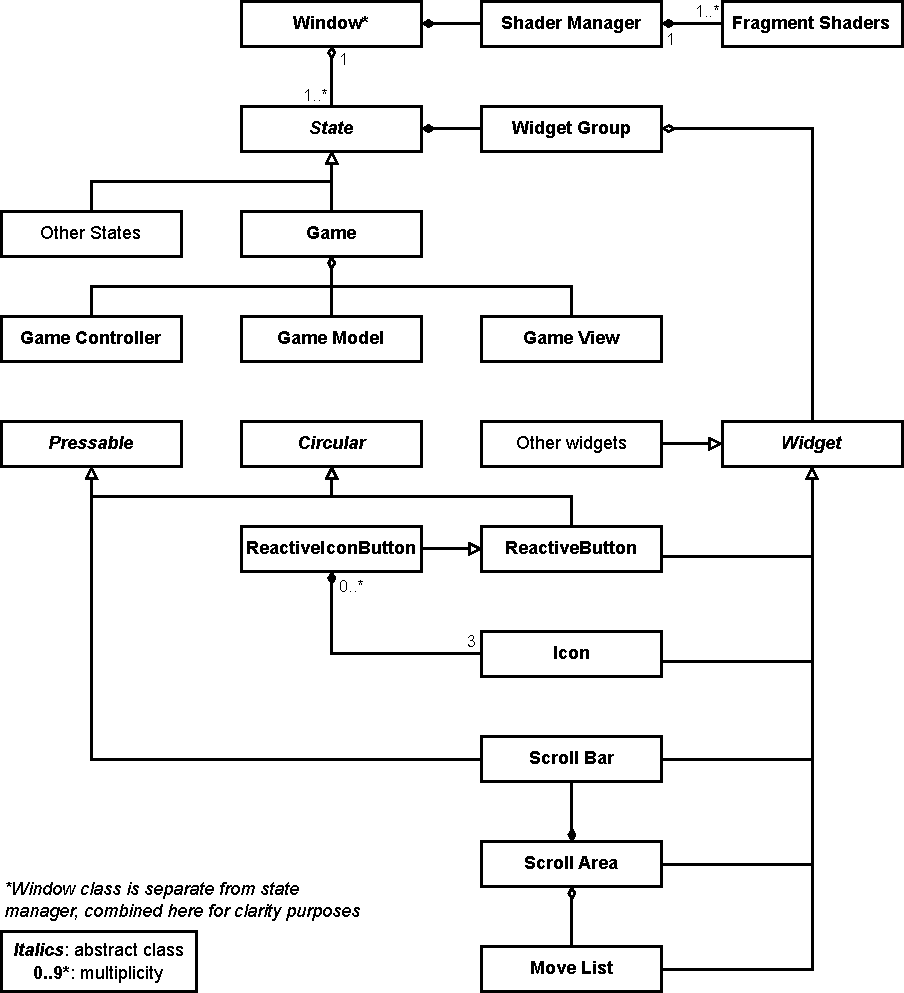
\includegraphics[width=\columnwidth]{../design/assets/class_relation_diagram.pdf}
    \label{fig:class-relation-diagram}
\end{figure}

\noindent View complete \href{https://raw.githubusercontent.com/TubTubTub/NEA/main/documentation/design/assets/documentation/design/assets/widgets_class_diagram.pdf}{class diagram for all widgets.}

\noindent View complete \href{https://raw.githubusercontent.com/TubTubTub/NEA/main/documentation/design/assets/documentation/design/assets/all_class_diagram_1}{class diagram for entire program.}

\noindent View \href{https://raw.githubusercontent.com/TubTubTub/NEA/main/documentation/design/assets/documentation/design/assets/all_class_diagram_2.pdf}{alternate class diagram for entire program.}

\noindent (Generated with \verb|Pyreverse|)

\end{document}